
%(BEGIN_QUESTION)
% Copyright 2011, Tony R. Kuphaldt, released under the Creative Commons Attribution License (v 1.0)
% This means you may do almost anything with this work of mine, so long as you give me proper credit

Imagine a situation where the PV signal pressure is 8 PSI and the SP signal pressure is 10 PSI:

$$\includegraphics[width=15.5cm]{i01761x01.eps}$$

Explain what the output pressure in this pneumatic controller will do over time so long as this imbalance between PV and SP persists.  Assume all bellows are equal in size (effective area), and that the fulcrum is precisely centered in the middle of the beam.

\vskip 10pt

Now, imagine a situation where the output pressure of this mechanism is 11 PSI, and at that exact moment the output pressure reaches 11 PSI, the setpoint pressure is suddenly reduced from 10 PSI to 8 PSI, so that now PV = SP.  Explain what effect this will have on the output pressure, both immediately and over time.

\vskip 20pt \vbox{\hrule \hbox{\strut \vrule{} {\bf Suggestions for Socratic discussion} \vrule} \hrule}

\begin{itemize}
\item{} A general problem-solving principle to apply to a problem such as this is a {\it force diagram}.  This means representing each and every active force in a mechanical system using arrows, showing both magnitude and direction.
\item{} How will the situation differ if the reset valve is opened just a bit more?
\item{} Why is there no bias spring in this mechanism?  Is this merely a simplification, or is there a deeper meaning to the spring's omission?
\end{itemize}

\underbar{file i01761}
%(END_QUESTION)





%(BEGIN_ANSWER)

\noindent
{\bf Partial answer:}

\vskip 10pt

When SP $>$ PV, the output pressure will steadily rise.

%(END_ANSWER)





%(BEGIN_NOTES)

When SP $>$ PV, the output pressure will steadily rise, with the output pressure leading the reset bellows pressure by a difference of 2 PSI.

\vskip 10pt

If the SP suddenly drops to equal the PV just as soon as the output pressure reaches 11 PSI (rising), the output pressure will suddenly drop to 9 PSI and hold steady (9 PSI inside the reset bellows as well).

\filbreak \vskip 20pt \vbox{\hrule \hbox{\strut \vrule{} {\bf Virtual Troubleshooting} \vrule} \hrule}

\noindent
{\bf Predicting the effect of a given fault:} present each of the following faults to the students, one at a time, having them comment on all the effects each fault would produce.

\begin{itemize}
\item{} Restrictor plugs
\item{} Valve plugs
\item{} Nozzle plugs
\item{} Reset bellows develops a major leak
\item{} Feedback (output) bellows develops a major leak
\item{} Air supply pressure increases
\end{itemize}


\vskip 10pt


\noindent
{\bf Identifying possible/impossible faults:} present symptoms to the students and then have them determine whether or not a series of suggested faults could account for all the symptoms, explaining {\it why} or {\it why not} for each proposed fault:

\begin{itemize}
\item{} Symptom: {\it }
\item{} 
\item{} 
\item{} 
\end{itemize}


\vskip 10pt


\noindent
{\bf Determining the utility of given diagnostic tests:} present symptoms to the students and then propose the following diagnostic tests one by one.  Students rate the value of each test, determining whether or not it would give useful information (i.e. tell us something we don't already know).  Students determine what different results for each test would indicate about the fault, if anything:

\begin{itemize}
\item{} Symptom: {\it }
\item{}  -- {\bf Yes/No}
\item{}  -- {\bf Yes/No}
\end{itemize}


\vskip 10pt


\noindent
{\bf Diagnosing a fault based on given symptoms:} imagine the ??? fails ??? in this system (don't reveal the fault to students!).  Present the operator's observation(s) to the students, have them consider possible faults and diagnostic strategies, and then tell them the results of tests they propose based on the following symptoms, until they have properly identified the nature and location of the fault:

\begin{itemize}
\item{} {\it }
\item{} 
\item{} 
\end{itemize}
%INDEX% Control, proportional + integral: pneumatic force-balance controller

%(END_NOTES)


